\documentclass{article}

\usepackage{amsmath}
\usepackage{amssymb}
\usepackage{amsthm}
\usepackage{amssymb}
\usepackage{mathdots}
\usepackage[pdftex]{graphicx}
\usepackage{fancyhdr}
\usepackage[margin=1in]{geometry}
\usepackage{multicol}
\usepackage{bbm}
\usepackage{esint}
\usepackage{listings}
\PassOptionsToPackage{usenames,dvipsnames}{color}  %% Allow color names
\usepackage{pdfpages}
\usepackage{algpseudocode}
\usepackage{tikz}
\usepackage[T1]{fontenc}
\usepackage{inconsolata}
\usepackage{framed}
\usepackage{wasysym}
\usepackage[thinlines]{easytable}
\usepackage{wrapfig}
\usepackage{hyperref}
\usepackage{cancel}
\usepackage{tabu}
\usepackage{tabularx}
\usepackage{mathtools}
\usepackage{mathrsfs}
\usepackage{enumerate}
\usepackage{enumitem}
\usepackage{tabto}

% Margins
\topmargin=-0.45in
\evensidemargin=0in
\oddsidemargin=0in
\textwidth=6.5in
\textheight=9.0in
\headsep=0.25in

\title{Problem Set 1}
\author{Laker Newhouse\\Collaborators: Evelyn Fu}
\date{\today}

\begin{document}
\maketitle	

All code and raw results are available at \url{https://github.com/Arongil/6.S098/tree/main/pset1}.
\begin{enumerate}
    \item (Bonds) The idea is to formulate a linear program which encodes the constraints on the price discounting. Then to find $d^\text{max}$ and $d^\text{min}$, we solve $2n$ linear programs of the form \begin{align*}
        & \text{max } [0 \cdots \pm 1 \cdots 0]^T p \\
        & \text{subject to } C^T p = b, \; Dp \geq 0,
    \end{align*} where $C$ is the bond matrix (rows are bonds, columns are payment schedule) and D is the matrix \[
        D = \begin{pmatrix}
            1 & -1 & 0 & \cdots & 0 & 0 \\
            0 & 1 & -1 & \cdots & 0 & 0 \\
            \vdots & \vdots & \vdots & \ddots & \vdots & \vdots \\
            0 & 0 & 0 & \cdots & 1 & -1 \\
            0 & 0 & 0 & \cdots & 0 & 1 \\
        \end{pmatrix},
    \] which serves to enforce both the nonincreasing and nonnegativity conditions. We graph the result. At two points (24 months and 60 months), our bounds converge to tell us exactly what the discount is.
    
    \begin{center}
    	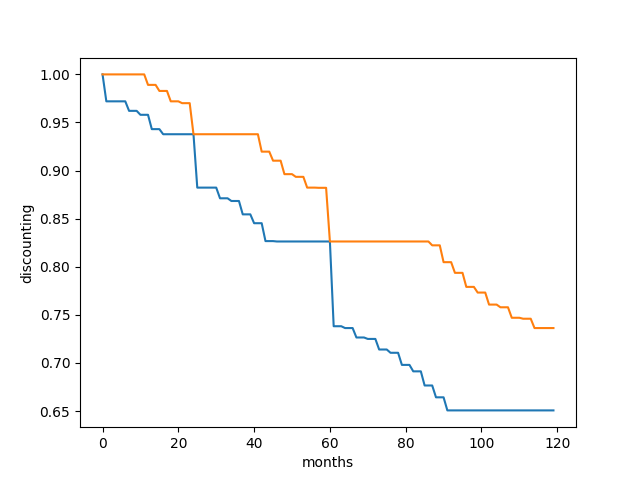
\includegraphics[scale=0.5]{p1_plot}
    \end{center}
    
    \item (Permutations) We use the constraints \begin{align*}
    	&P \geq 0, \\
    	&P \mathbbm{1} = \mathbbm{1}, \\
    	&P^T \mathbbm{1} = \mathbbm{1}, \\
    	&P A = B P,
    \end{align*} where the final constraint rewrites $PAP^T = B$, recalling that $P^T = P^{-1}$ for permutation matrices. \\

	The resulting permutation vector is (6. 22. 27. 19. 15.  3. 11. 25. 21. 23.  9.  4. 26. 16. 12. 17. 30.  1. 20.  7.  5. 24. 18.  8. 10. 13.  2. 28. 14. 29.) For proof that matrix elements were near to integers, we report $\max p_{ij}(1 - p_{ij}) = 1.87 \times 10^{-10}$.
    
    \item (Reformulations) We present our reformulations. We have tested each and successfully shown them all to be DCP. \begin{enumerate}
    	\item Use constraints $x \geq 0, y \geq 0, cp.harmonic\_mean(cp.hstack([x, y])) \geq 2$.
    	\item Use constraints $x \geq 0, y \geq 0, cp.inv\_prod(cp.hstack([x, y])) \leq 1$.
    	\item Use constraints $y \geq 0, cp.quad\_over\_lin(x + y, cp.sqrt(y)) \leq x - y + 5$.
    	\item Let $GM(x, y)$ denote $cp.geo\_mean(cp.hstack([x, y]))$. \\
    	Use constraints $x \geq 0, y \geq 0, x + z \leq 1 + GM(GM(x, y) - z, GM(x, y) + z)$.
   	\end{enumerate}
   
   \item (Runtime) We report the desired data in a table. From top to bottom, the rows are for the exponential, linear, and built-in constraints. From left to right, the columns are for $n = 2, 5, 10$.
   \begin{center}
   	\begin{tabular}{ | m{1.5cm} | m{1.5cm}| m{1.5cm} | } 
   		\hline
   		0.000016 & 0.000074 & 0.004215 \\ 
   		\hline
   		0.000018 & 0.000031 & 0.000046 \\ 
   		\hline
   		0.000022 & 0.000030 & 0.000047 \\ 
   		\hline
   	\end{tabular}
   \end{center}
    
\end{enumerate}

\end{document}
